\chapter{Ontology Construction and Similarity}


We notice that simple keywords matching is not a good similarity measure, because job description and resume are both written in human language, even one concept, they could be written in different ways, and and some different concepts have a close relationship. For example, Table~\ref{tab:resume_jd}  is part of the resume of a job seeker, and part of a job description:

\begin{table}[ht]
\caption{Resume and Job Description} % title of Table
\centering % used for centering table
\begin{tabular}{ | p{8cm} | p{7cm} | }
 \hline
   \textbf{Part of Resume}                 &   \textbf{Part of Job Description}   \\ \hline

    B.S. degree in computer science \newline
    5+ years Java \newline
    2+ year   C++  \newline
    Some experience in Oracle database \newline
    Other experience like: \newline
    Hibernate, JBOSS, JUnit, Tomcat etc.
  &
  BS degree above   \newline
  4+ years Java  \newline
  Some experience of Python   \newline
    Mysql, MS-SQL   \newline
    Java web application Server   \newline
    OOA/OOD   \\
 \hline
\end{tabular}
\label{tab:resume_jd} % is used to refer this table in the text
\end{table}

If just looking at the text, we can find the resume has few common words with the job description. But from the view of an experienced engineer, the candidate is pretty matching the job. Because relational databases Oracle and Mysql are very similar, OOA/OOD is the same meaning of many years of Java and C++ experience, and Tomcat and JBOSS are two Java web applications servers.  If we use key word matching, the system won't give a good matching result in this very common situation. 

\subsection{Semantic Similarity in JRSs}
We had studied previous work on similarity measures in JRSs, some of them use ontology to store knowledge and rules, also aid information extraction. Liu and Dew~\cite{liu2004using} used RDF to represent and store the expertise of experts , and a RDF-based Expertise Matcher could retrieves the experts whose expertise include the required concept.

Proactive~\cite{lee2007fighting} used two kinds of ontology, job category and the company information. The system used ontology checker to classify the job information, stored the domain knowledge and calculated the weight value in recommendations. 


Fazel \cite{fazel2009semantic} used a hybrid approach to matching job seekers and job postings, which takes advantage of the benefits of both logic-based and ontology-based matching. In his paper the description logics (DL) is used to represent the candidate and job opening, and the ontology is used to organize the skills in a skill taxonomy. He gave an equation to calculate  the matching degree:
$$ sim\left(P ,j \right) = \sum x_{ij} \times u(ds_i) $$

where, $x_{ji}$ is the Boolean variable indicating whether desire i is satisfied by applicant $A_{j}$ in the set of all qualified applications.

Kumaran et al~\cite{kumaran2013towards} also used ontology to calculate the similarity between job criteria and candidates's resume in their system~\cite{kumaran2013towards}. The similarity equation they used are:
$$ M\left ( i_1, i_2 \right ) = \frac{\sum_{k=1}^{n} Sim\left (p_{k}^{i1},  p_{k}^{i2} \right ) * W_{k}^{i2}}{\sum_{k=1}^{n} W_{k}^{i2}}  $$
The similarity function $Sim(p_1, p_2)$ is defined as follows:
$$ Sim(p1, p2) = \begin{Bmatrix}
1, & if~similarity~of~p1~and~p2 \geqslant t\\
0, & otherwise
\end{Bmatrix} $$



\section{Ontology Construction}

\subsection{Domain Specific Ontology}
Before calculate the similarity between concepts, we need construct the Ontology at first. Semantic web have been a hot research topic in these years, thousands of domain ontologies had created~\cite{ding2004swoogle}. A paradigmatic example is WordNet~\cite{fellbaum1998wordnet}, is a general purpose thesaurus, that contains more than 100,00 general English concepts. ACM has created a poly-hierarchical ontology that can be utilized in semantic web applications~\cite{acm2012class}, but it is mostly used in academic area. Currently, there is no IT technology ontology build for recruiting purpose.

The IT ontology for recruiting should include a lot of technical terms, like programming language, programming library, commercial products and so on. Furthermore there are new techniques invented everyday, so new IT terms will appear continuously. Ding et al.~\cite{ding2002ontology} give a survey of current ontology generation approaches, such as manual, semi-automatic, and automatic. Some aspects the approaches had been discussed in the paper, like the source data, concept extraction methods, Ontology representation, and construction tools. Inspiring on this paper, we used semi-automatic approach to construct the IT skill ontology.

From the observation, we found that  skills requirement part of job description always list several skills in one the sentence, which is shown in table ~\ref{tab:skillrequirement}. Based on this character, we propose a bootstrap approach to collect IT terms in job descriptions. We first manually collect about fifty terms from job descriptions, and add them to the term list. Then we use our pattern matching tools to find tokens matching some patterns in table \ref{tab:patterns}.  The terms we get have high probability to be technical terms. Then we could check the words in Dbpedia to check whether they are under the categories like software, programming language or any other technical related ones. If they are, we could classify them as terms, and add them to the terms list. 

\begin{table}[ht]
\caption{Some sentences Job Description} % title of Table
\centering % used for centering table
\begin{tabular}{ | p{15cm}  | }
 \hline
    1. A high-level language such as Java, Groovy, Ruby or Python; we use Java and Groovy extensively \newline
    2. HTML5/CSS3/JavaScript, web standards, jQuery or frameworks like AngularJS would be great \newline
    3. HTML CSS and Javascript a must  \newline
    4. Experience with AJAX, XML, XSL, XSLT, CSS, JavaScript, JQuery, HTML and Web Services   \\
 \hline
\end{tabular}
\label{tab:skillrequirement} % is used to refer this table in the text
\end{table}



\begin{table}[ht]
\caption{Patterns to extract terms} % title of Table
\centering % used for centering table
\begin{tabular}{   | p{8cm} |  }
 \hline
     term   , * , *,  term  \\  \hline
     term  , * , *, and  term   \\
 \hline
\end{tabular}
\label{tab:patterns} % is used to refer this table in the text
\end{table}

\begin{table}[ht]
\caption{Some sentences Job Description} % title of Table
\centering % used for centering table
\begin{tabular}{   | c | c | c | c |c | c |c | c |c | c |c | c |c | c |  }
 \hline
     Experience & with & TERM & , & *   & , & *   &, & TERM &, & and & *  \\
 \hline
     Experience & with & AJAX & , & XML & , & XSL &, & XSLT &, & and & CSS  \\
 \hline
\end{tabular}
\label{tab:termspattern} % is used to refer this table in the text
\end{table}

For example, we extract the word  ''XSL'', which currently not in the skill set. We check the word on DBpedia, get the XML formatted description from URL : http://dbpedia.org/page/XSL. If any element in ``dcterms:subject'' has the value which is the technical category,  like ``Programming languages'', ``Markup languages'', we can indicate that the word is a technical term, and pop them up. Such iteration will continue until the number of new terms getting below a threshold. The process is shown Figure ~\ref{fig:gen_onto}

\begin{figure}[htbp]
  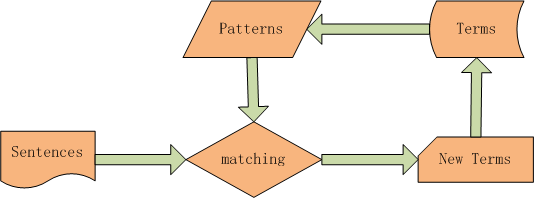
\includegraphics[scale=0.6]{images/genonto.png}
  \caption{Find Technical Terms}
  \label{fig:gen_onto}
\end{figure}

After getting all terms, we use Protege~\cite{noy2001creating}, an open source ontology editor, to create the domain specific ontology, save as RDF format. It's interface of Protege is shown in Figure~\ref{fig:Protege}. Part of the technical ontology is shown in Figure ~\ref{fig:ontology_pro}.


\begin{figure}[htbp]

  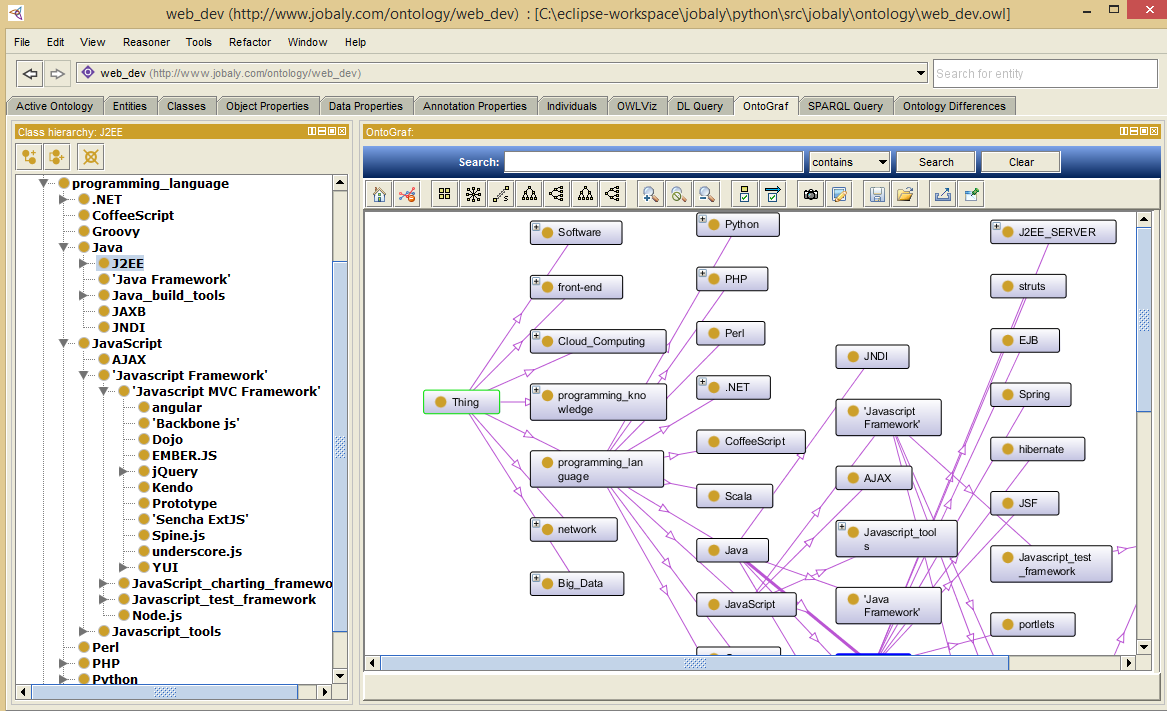
\includegraphics[scale=0.5]{images/protege.png}
  \caption{Interface of Protege}
  \label{fig:Protege}
\end{figure}

\begin{figure}[htbp]

  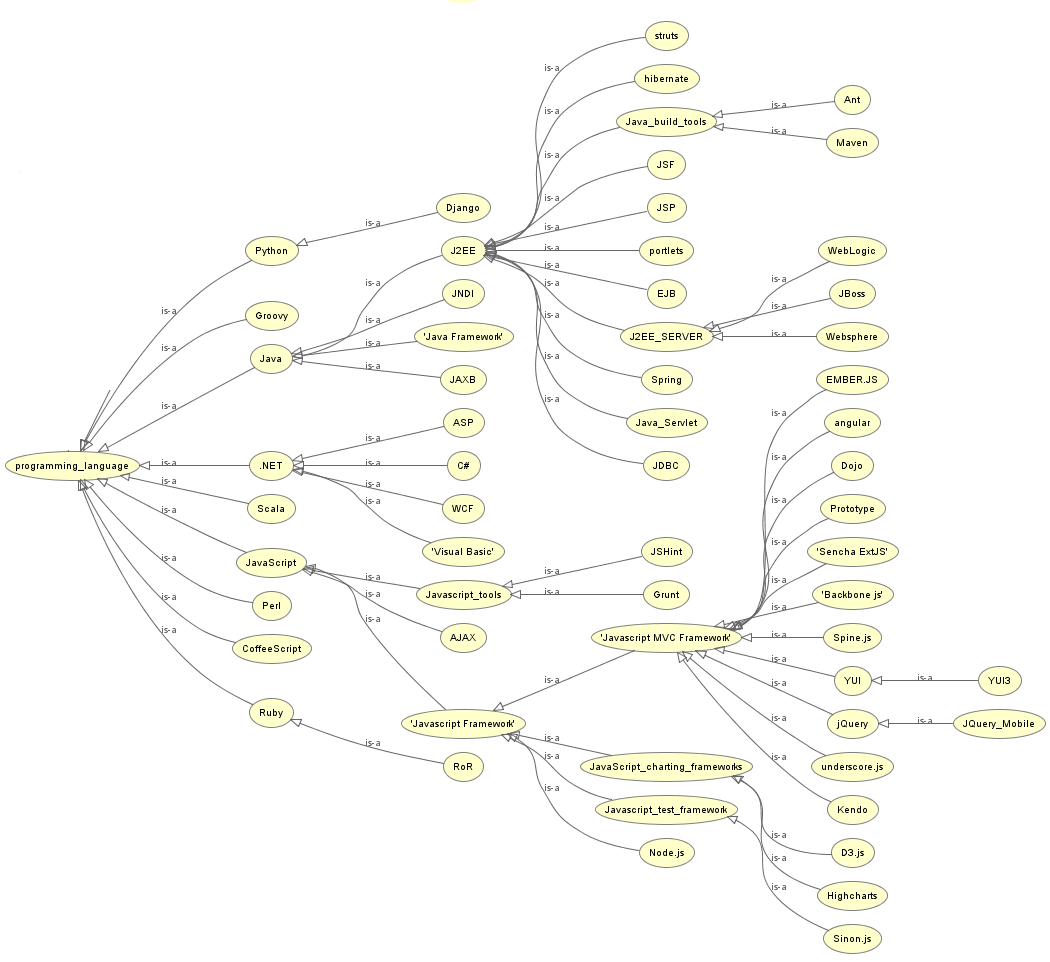
\includegraphics[scale=0.6]{images/ontology_pro.png}
  \caption{Part of Ontology}
  \label{fig:ontology_pro}
\end{figure}

\section{Ontology-based semantic similarity}

The Ontology technics had also been used in some JRSs, which provide a formal specification of a shared conceptualization~\cite{guarino1998formal}. S{\'a}nchez et al. \cite{sanchez2012ontology} summarized ontology-based similarity assessment into three kinds, and advantages and disadvantages of each approach. The three kinds of categories are: Edge-counting approaches, Feature-based measures, and Measures based on Information Content.


\subsection{Path-based approaches}
In path-based approaches , the ontology is viewed as a directed graph, in which the nodes are the concepts, the edges are taxonomic relation, like (is-a). Rada, et al.,~\cite{rada1989development} measure the similarity by the distance of two nodes in the graph. So the semantic distance of two concepts a and b will be:
$$ dis_{rad}(a,b) = min |path_i(a,b)| $$

Wu and Palmer ~\cite{wu1994verbs} realized that the depth in the taxonomy will impact the similarity measure of two nodes, because the more deeper of the nodes are in the tree, the semantic distance is smaller. So they gave a new measure of ontology:
$$ sim_{w\&p}(a,b) = \frac{2 \times N_3}{N_1 + N_2 + 2 \times N_3} $$
$N_1$ and $N_2$ is the numbers of is-a links from each term to their Least Common Subsumer(LCS), $N_3$ is the number of is-a links of the LCS to the root of the ontology.

Based on the same idea, Leacock and Chodorow~ \cite{leacock1998combining} also proposed similarity measure that combined distance Np between terms a and b and the depth $D$ of the taxonomy.
$$ sim_{l\&c}(a,b) = -\log (Np/ 2D) $$

There are some limitations of path-based approaches. First it only consider the shortest path between concept pairs, when they meet complex situation like multiple taxonomical inheritance, the accuracy of them will be low.  Another problem of path-based measures assume that all links in the taxonomy have uniform distance.

\subsection{Feature-based measures}

Feature based approaches assess similarity between concepts as a function of their properties. They consider degree of overlapping between sets of ontological features, like Tversky's model~\cite{tverskyfeatures}, which subtract the non-common features from common features of two concepts.
$$  sim_{tve}(a,b) = \alpha \cdot F \left( \Psi(a) \cap   \Psi(b)  \right) - \beta  \cdot F \left( \Psi(a) \setminus   \Psi(b)  \right) - \gamma \cdot F \left( \Psi(b) \setminus   \Psi(a)  \right)  $$
Where F is salience of a set features, and $\alpha, \beta$ and $\gamma$ are weights of the contribution of each component.

Rodr{\'\i}guez and Egenhofer~\cite{rodriguez2003determining} computed similarity by sum the weighted sum of similarities between synsets, features, and neighbour concepts.
$$ sim_{re}(a,b) = w \cdot S_{synsets}(a,b) + u \cdot S_{features}(a,b) + v \cdot S_{neighborhoods}(a,b) $$

The feature-based methods consider more semantic knowledge than path-based methods. But only big ontologies/thesauri like Wordnet~\cite{miller1995wordnet} have this kind of information. Ding et al.~\cite{ding2004swoogle} had revealed that domain ontologies very occasionally model any semantic feature apart from taxonomical relationship.

\subsection{Content-based measures}
Other approaches want to overcome the limitations of edge-counting approaches are Content-based measures. Resnik~\cite{resnik1995using} proposed similarity, which depends on the amount of shared information between two terms:
$$ sim_{res}(a,b) = IC(LCS(a,b))$$
LCS is the Least Common Subsumer of terms in a ontology, and IC is Information Content, which is the negative log of its probability of occurrence, $p(a)$. Lin (1998) and Jiang and Conrath (1997) extended Resnik��s work. They also considered the IC of each of the evaluated terms, and they proposed that the similarity between two terms should be measured as the ratio between the amount of information needed to state their commonality and the information needed to fully describe them.
$$ sim_{lin}(a,b)=\frac{2 \times sim_{res}(a,b)}{(IC(a)+IC(b))}$$
The are also two disadvantages of content-based measures. First these approaches cannot compute the concepts of leave nodes, because they don't have subsumers. Second if the concepts do not have enough common subsumers,their similarities are hard to be calculated.


\section{Statistical-based Ontology Similarity Measure }
In this thesis, I proposed a new statistical-based ontology similarity measure. In most of job descriptions, they will list many skills the positions required.  From observation, we found that related skills always exist in the job description simultaneously, and the positions of them are always close, e.g. HTML and CSS are always required together, and appear in the same sentence. We could see this phenomenon in table~\ref{tab:skillinsent}, which include some skills requirement sentences from some job descriptions.

\begin{table}[ht]
\caption{Some sentences Job Description} % title of Table
\centering % used for centering table
\begin{tabular}{ | p{15cm}  | }
 \hline
    1. A high-level language such as Java, Groovy, Ruby or Python; we use Java and Groovy extensively \newline
    2. HTML5/CSS3/JavaScript, web standards, jQuery or frameworks like AngularJS would be great \newline
    3. HTML CSS and Javascript a must  \newline
    4. Experience with AJAX, XML, XSL, XSLT, CSS, JavaScript, JQuery, HTML and Web Services   \\
 \hline
\end{tabular}
\label{tab:skillinsent} % is used to refer this table in the text
\end{table}

We could see from the table, the technical close related concepts are always have short distance. Based on such observation, we give a new statistical-based ontology similarity measure. Similarity between two concepts can be calculated,  if the two concepts $a$ and $b$ have the same direct hypernym or one  is the hypernym of the other. Their similarity $S_{a,b}$ could be the ratio between two factors:

\begin{enumerate}
    \item The ratio of the number of documents they exist together $N_{a \cap b}$ to the number of documents have a least one them $N_{a \cup b}$.
    \item The average $\log$ value of their minimum distance $mindis(doc,a,b)$ in documents that have them both.
\end{enumerate}

$$ S(a,b) = \frac{  N_{a \cap b} / N_{a \cup b} }{avg(\log_2( mindis(doc,a,b) + 1 ))} $$

If distance between two concepts are further than above situation we generally believe they are not related skills. We set the restriction because the position of the concepts in the ontology are based on their technical similarity to others. Similar techniques will assigned into a same category, they should share the same technology base, and one could be a alternate or similar to the other. For example, we put EJB and Hibernate in the same category, because they are both J2EE persistence layer technologies, and both have the O/R mapping concept. If the applicant is familiar one of them, they can master the other very quickly. Another example, like Grail and Django, they are both web frameworks, and share some web design philosophies, but one is  designed for Java web application and the other is created for Python web application. So if one developer has some some experience with one of them, he/she still need spend a lot of time to learn the other to overcome the gap between programming languages. The algorithm to calculate the similarity of two concepts is in algorithm ~\ref{alg:alg_similarity}.

\begin{algorithm}
\caption{Get Stat Similarity}
\label{alg:alg_similarity}
\KwIn{$Docs$�� $term1$, $term2$}
\KwOut{$similarity$}
$total=0$;
$hastwo=0$;
$dislist=\left [ ~~ \right ]$\;
\For{$i=1;~i~\le~len(Docs);~i++$}
{
  \If{ $ Docs_i~has~at~least~one~term $ }
    {
     $ total~+=~1 $ \;
     \If{ $ Docs_i~has~both~terms $ }
        {
           $ hastwo~+=~1 $ ;
           $ mindis~=~ minimium\_distance~(Docs_i, term1, term2) $ \;
           $ dislist.~add  ~\left(  log_2( mindis + 1 ) \right) $ \;
        }
    }
}
$ factor1~=~hastwo~ /~ total $  \;
$ factor2~=~ avg(dislist) $  \;
return $factor1 ~/~ factor2$\;
$ ~~ $
\end{algorithm}

We got the relevance matrix in table~\ref{tab:dismatrix1} by using the algorithm from 500 job descritptions. Considering the skill HTML, the most relevance skills in order are CSS, Javascript, and jQuery,  which is the same from the perspective of a experienced developer. The other example is Java, the most relevant skill in the matrix is JSP, which is also agree with the general technical knowledge.


\begin{table}

\caption{Skills Similarity Table 1}
\begin{tabular}{ c | c c c c c c   }
 \hline
  Term       &  Java  &  JDBC  & Spring & Hibernate & MySql  & Oracle   \\  \hline
  Java   &   1    & 0.0523 & 0.091  &   0.0458  & 0.0339 & 0.0608    \\  \hline
    JDBC   & 0.0523 &   1    & 0.0525 &   0.0799  & 0.006  & 0.0616   \\  \hline
   Spring  & 0.091  & 0.0525 &   1    &   0.2008  & 0.0194 & 0.0878   \\  \hline
 Hibernate & 0.0458 & 0.0799 & 0.2008 &     1     & 0.0073 & 0.115    \\  \hline
   MySql   & 0.0339 & 0.006  & 0.0194 &   0.0073  &   1    & 0.049    \\  \hline
   Oracle  & 0.0608 & 0.0616 & 0.0878 &   0.115   & 0.049  &   1      \\  \hline
 \hline
\end{tabular}
\label{tab:dismatrix1}
\end{table}


\begin{table}

\caption{Skills Similarity Table 2 }
\begin{tabular}{ c | c c c c c c c c }
 \hline
  Term       & Javascript & jQuery &  HTML  &  CSS   &  Java  & Python &  Ruby  &  JSP    \\  \hline
  Javascript &     1      & 0.1981 & 0.2087 & 0.2439 & 0.0665 & 0.0189 & 0.023  & 0.0253   \\
    jQuery   &   0.1981   &   1    & 0.0979 & 0.1328 & 0.0439 & 0.0142 & 0.0266 & 0.0232    \\
     HTML    &   0.2087   & 0.0979 &   1    & 0.3569 & 0.0473 & 0.0175 & 0.023  & 0.0103   \\
     CSS     &   0.2439   & 0.1328 & 0.3569 &   1    & 0.0537 & 0.0153 & 0.0181 & 0.015    \\
     Java    &   0.0665   & 0.0439 & 0.0473 & 0.0537 &   1    & 0.0498 & 0.0287 & 0.075    \\
    Python   &   0.0189   & 0.0142 & 0.0175 & 0.0153 & 0.0498 &   1    & 0.1333 & 0.0025   \\
     Ruby    &   0.023    & 0.0266 & 0.023  & 0.0181 & 0.0287 & 0.1333 &   1    & 0.012    \\
     JSP     &   0.0253   & 0.0232 & 0.0103 & 0.015  & 0.075  & 0.0025 & 0.012  &   1      \\
 \hline
\end{tabular}
\label{tab:dismatrix2}
\end{table}

\section{Combine Keyword Search and Ontology Matching }

Using ontology matching, the system can give job seekers some jobs appropriate to their background. But in some cases, job seekers have their own preference when choosing jobs. These cases are not very rare, for example, some people may want to try some new positions or industries they have no or few experience, because they are boring with current positions, or they want to learn some perspective technologies. Considering such situation, we add a new search function to the system, which combine the traditional keyword searching and our ontology matching approach. At first users need to upload their resume, and then they can use keywords to search jobs. The system will get the jobs that contain the keywords, and the jobs are ranked by their similarity values to the users' resume. The keywords represent user's preference, that jobs satisfied this criteria will be returned, and the ontology similarity become the ranking algorithm, which make the top items of the searching result more relevance to user.
